\documentclass[twocolumn,11pt]{article}
\usepackage[margin=2cm]{geometry}
\usepackage{amsmath,amsfonts,amssymb}
\usepackage{graphicx}
\usepackage{natbib}
\usepackage{url}
\usepackage{lineno}
\usepackage{setspace}
\usepackage{xcolor}
\usepackage{soul}
\usepackage{subcaption}

% Title and authors
\title{\textbf{Paleomagnetic and Geochemical Investigation of the Bolaven Plateau Volcanic Field: Testing the Australasian Impact Crater Hypothesis, Southern Laos}}

\author{Nicolas Anderson\textsuperscript{1,*}, Paolo Sanchez\textsuperscript{1}, Kerry Sieh\textsuperscript{2}, and Joseph L. Kirschvink\textsuperscript{1}\\
\small \textsuperscript{1}Division of Geological and Planetary Sciences, California Institute of Technology, Pasadena, CA 91125, USA\\
\small \textsuperscript{2}Earth Observatory of Singapore, Nanyang Technological University, Singapore 639798\\
\small *Corresponding author: nanderson@caltech.edu}

\date{}

\begin{document}

\maketitle

\begin{abstract}
The source crater for the Australasian tektite strewn field, formed by a large bolide impact at approximately 790 ka, has remained elusive for over a century despite extensive searches across Southeast Asia. Recent geological, geochemical, and geophysical evidence suggests that this impact crater lies buried beneath the basaltic lavas of the Bolaven Plateau volcanic field in southern Laos. To test this hypothesis, we conducted the first detailed paleomagnetic and magnetostratigraphic study of the Bolaven volcanic field, analyzing approximately 80 drill core and block samples from 16 localities across southern Laos. Our investigation included vibrating sample magnetometer (VSM) analysis, thermal and alternating field demagnetization, conglomerate tests on proposed ejecta deposits, and polarity determinations of propsoed in-situ basalt flows. Our results reveal that weathered basalt surfaces show consistently lower coercivity (###) but higher remanent (###) and saturation magnetization (###) compared to fresh cores, indicating maghemite as the dominant magnetic carrier in weathering rinds. Conglomerate tests confirm that 8 of 9 interpreted in-situ basalt sites failed the test as expected, while 3 of 4 ejecta deposits passed, supporting their interpretation as impact debris. Magnetic polarities agree well with \textsuperscript{40}Ar/\textsuperscript{39}Ar ages for most in-situ flows, providing some magnetostratigraphic constraints. One previously interpreted in-situ flow (PKS-HA) passed the conglomerate test, suggesting it is actually an ejecta deposit, not an insitu flow. These results provide the first paleomagnetic evidence supporting the Bolaven Plateau impact hypothesis and demonstrate the utility of rock magnetic techniques for distinguishing impact ejecta from in-situ volcanic flows.
\end{abstract}

% Two-column spanning figure
\begin{figure*}[htbp]
    \centering
    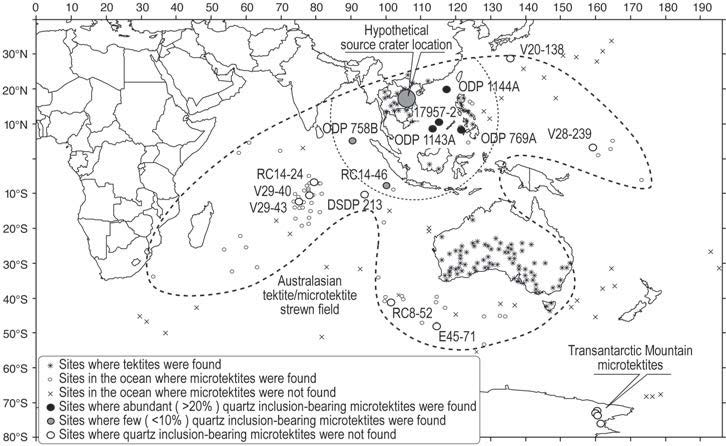
\includegraphics[width=0.8\textwidth]{folco_2010_tektite_map.jpeg}
    \caption{Australasian tektite and microtektite strewn field (dashed line; Glass and Koeberl, 2006). Sites where microtektites containing quartz inclusions were found are labeled. Dotted line encloses sites where shocked quartz and coesite were found within microtektite layer (Glass and Wu, 1993). Sites where Transantarctic Mountain microtektites were found are also shown (Folco et al., 2008, 2009). They likely represent southeastern extension of Australasian strewn field and they do not contain quartz inclusions. Figure and caption modified from \citet{Folco2010}.}
    \label{tektite_map}
\end{figure*}

\section{Introduction}

The Australasian tektite strewn field represents one of the most extensive impact ejecta deposits on Earth, covering approximately 20\% of the Earth's eastern hemisphere from Indochina to East Antarctica \citep{Glass1994}. These glassy impact spherules, formed by a bolide impact at 790 $\pm$ 3 ka \citep{Schwarz2016, Jourdan2019}, provide compelling evidence for a major impact event during the late Pleistocene. Despite nearly a century of searching, the source crater for these tektites has remained one of the most enduring mysteries in impact geology.

The northwest-trending increase in both abundance and size of tektite specimens points to an impact site in eastern central Indochina \citep{Glass1994, Ford1988}. Geochemical analysis of the tektites indicates target rocks consisting primarily of quartz-rich coarse siltstone to fine sandstone, with evidence for a mafic component \citep{Koeberl1992, Wasson1991}. The high silica content, relict mineral grains, and elevated concentrations of elements such as Mg, Ni, Co, and Cr suggest mixing of siliciclastic sediments with basaltic materials \citep{Amare2006, Goderis2017}.

Recently, \citet{Sieh2019} presented compelling evidence that the Australasian impact crater lies buried beneath the Bolaven Plateau volcanic field in southern Laos. Their hypothesis is supported by five lines of evidence: (1) tektite geochemistry consistent with mixing of local sandstone and basaltic materials, (2) pre- and post-impact basaltic flows for the right age that could bury the crater, (3) a negative gravity anomaly of appropriate dimensions within the volcanic field, (4) proximal ejecta deposits with shocked quartz, and (5) the capping massive silty deposit, which contains microscopic tektite spherules termed “catastro-loess” or Bolaven diamicton.

The timing of the Australasian impact at 790 ka is particularly significant as it barely predates the Brunhes-Matuyama (BM) polarity reversal at 773 $\pm$ 3 ka \citep{Singer2019}. This proximity to a major geomagnetic field reversal provides an opportunity to investigate potential relationships between large impacts and geomagnetic field behavior. Previous studies have suggested that major impacts might influence geodynamo processes \citep{Muller1986}, though this remains controversial.

\hl{Paleomagnetic analysis offers powerful tools for testing the Bolaven impact hypothesis. Magnetostratigraphic polarity determinations can help confirm wwher dating can constrain the timing of volcanic activity relative to the impact, while analysis of remanent magnetization in ejecta deposits can reveal shock-related magnetic signatures. Furthermore, the temporal proximity to the BM reversal allows investigation of magnetic field behavior during this critical period.

Here we present the first comprehensive paleomagnetic and magnetostratigraphic study of the Bolaven Plateau volcanic field, combined with advanced geochemical modeling, to test the Australasian impact crater hypothesis and investigate associated magnetic field changes.}

\section{Geological Context}

\subsection{Regional Geology}

The Bolaven Plateau rises approximately 1 km above the surrounding Khorat Plateau in southern Laos, east of the Mekong River \citep{Sieh2019}. The plateau is underlain by nearly flat-lying Mesozoic quartz sandstones and mudstones of Jurassic age, which crop out almost continuously around the plateau's cliffy perimeter. These fine-grained siliclastic rocks comprise a 500-m-thick sequence, with the uppermost 200-250 m consisting of massive to cross-bedded fluvial sandstones overlying approximately 250 m of friable mudstones. Above the mudstoned are 

The Khorat Plateau represents the largest contiguous expanse of fine-grained, siliclastic Mesozoic sedimentary rocks in the region, covering approximately 155,000 km\textsuperscript{2}. 

% Two-column spanning figure
\begin{figure*}[htbp]
    \centering
    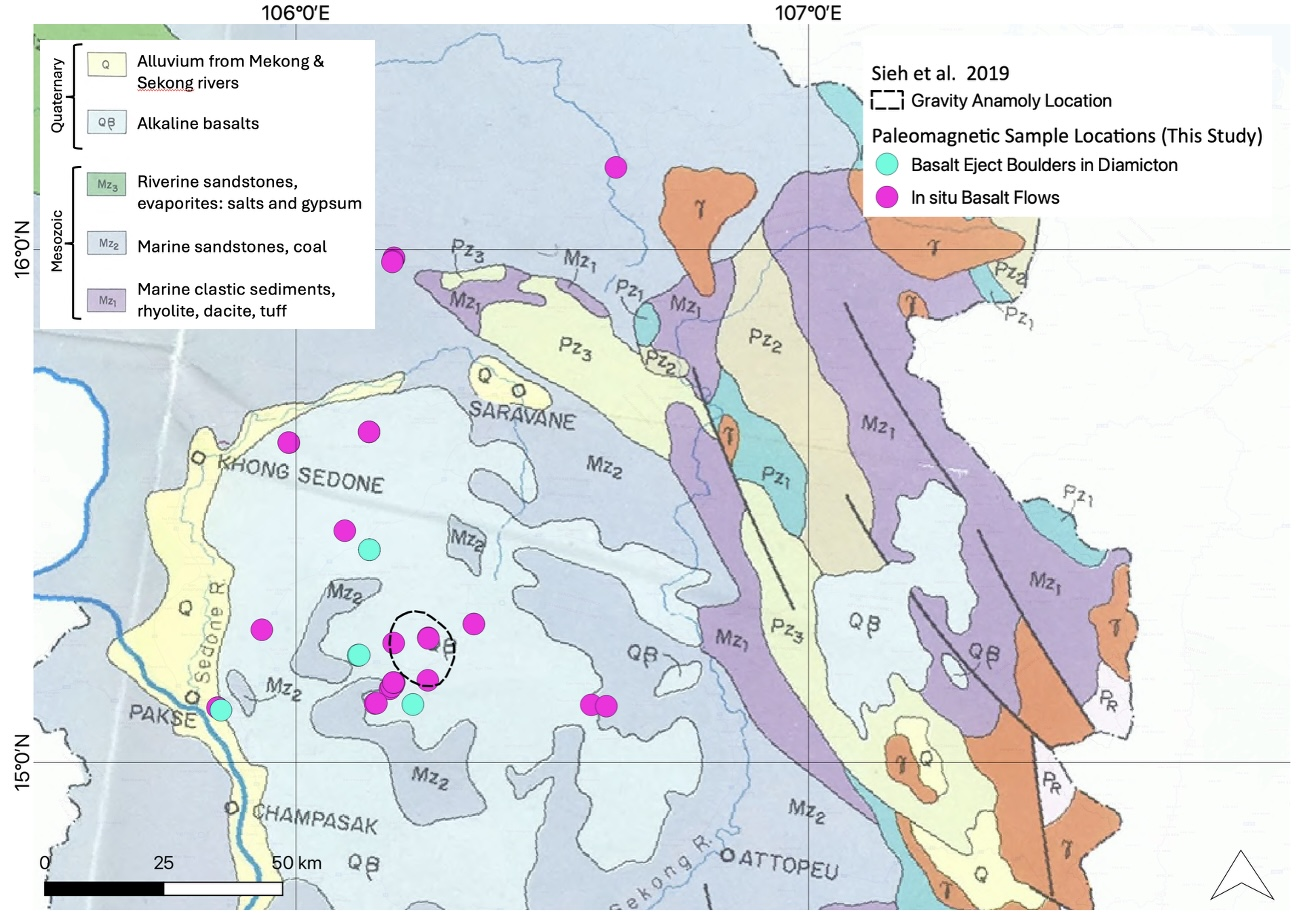
\includegraphics[width=0.8\textwidth]{sample_locations.jpg}
    \caption{Map of southern Laos, highlighting the locations of paleomagnetic sample sites from this study, both interpreted basaltic ejecta boulders and in-situ basalt flows. The map also highlights the location of the proposed crater location from Bouguer gravity anomaly data produced by \citet{Sieh2019}. Relevant Mesozoic and Quaternary units are shown. Figure modified from 1998 Laotian Government map.}
    \label{sample_locations}
\end{figure*}

\subsection{Bolaven Volcanic Field}

A basaltic volcanic field covering approximately 5,000 km\textsuperscript{2} caps the Mesozoic rocks and extends down the flanks of the plateau \citep{Sieh2019}. The volcanic field has a calculated volume of approximately 910 km\textsuperscript{3}, with basalt thickness reaching up to 300 m in the summit region. This extent and thickness are sufficient to completely obscure an impact crater up to 15 km in diameter with a rim rising several hundred meters above the bedrock surface.

The Bolaven volcanic field represents a typical intraplate basaltic field, characterized by scattered, low-eruption-volume scoria cones and flows reflecting the rise of individual batches of magma \citep{Valentine2010}. The field lacks the long-lived, localized composite volcanoes that would indicate the presence of a large crustal magma reservoir, making the existence of a buried caldera unlikely.

Previous \textsuperscript{40}Ar/\textsuperscript{39}Ar dating has revealed that volcanic activity spanned from approximately 16 Ma to 27 ka, with eruptions occurring both before and after the 790 ka impact \citep{Sieh2019, Sanematsu2011}. The temporal distribution of dated flows shows that most exposed lavas in the summit region are younger than the impact age, supporting the burial hypothesis. Additionally, the sedimentary sequences and the basaltic component provides an ideal target lithology matching the geochemical composition inferred from Australasian tektites \citep{Blum1992, Koeberl1992, Sieh2019}.

\subsection{Evidence for Impact}

\citet{Sieh2019} presented multiple lines of evidence supporting the presence of a buried impact crater beneath the Bolaven volcanic field:

\textbf{Geochemical evidence:} Principal component analysis of Australasian tektites indicates that $>$90\% of observed chemical variation can be explained by mixing of Mesozoic bedrock with Bolaven basalts and their weathered derivatives. The high \textsuperscript{10}Be concentrations in tektites are consistent with incorporation of meteoric \textsuperscript{10}Be from weathered basaltic saprolites.

\textbf{Geochronological constraints:} \textsuperscript{40}Ar/\textsuperscript{39}Ar dating reveals that all flows directly above the proposed crater center are younger than 790 ka, while pre-impact flows exist on the periphery of the field. This distribution supports complete burial of the impact site by post-impact volcanism.

\textbf{Geophysical anomaly:} A negative Bouguer gravity anomaly of approximately 6 mGal in the summit region corresponds to the expected signature of a buried crater filled with low-density impact breccia.

\textbf{Proximal ejecta:} A unique outcrop 10-20 km southeast of the proposed crater center exposes a sequence of brecciated sandstone and mudstone with features consistent with impact ejecta, including stratigraphic inversion, jigsaw-puzzle fitting of clasts, and shocked quartz grains with planar deformation features.

\subsection{Paleomagnetic Context}

The timing of the Australasian impact at 790 ka places it within a period of significant geomagnetic field variability leading up to the Brunhes-Matuyama reversal. \citet{Singer2019} documented field weakening beginning around 795 ka, followed by unstable polarity and intensity behavior around 785 ka, culminating in the final reversal to normal polarity at 773 ka. This temporal framework provides an important context for interpreting paleomagnetic results from the Bolaven field.

Impact-related magnetization can result from several processes, including shock remanent magnetization (SRM) acquired during the brief period of impact-induced shock compression, and thermoremanent magnetization (TRM) from impact-generated melts \citep{Tikoo2015}. These signatures, combined with detailed magnetostratigraphy, can provide crucial tests of the impact hypothesis.

\section{Methods}

\subsection{Sample Collection and Preparation}

Field work was conducted in southern Laos during November 2023, following approval from the Laotian Ministry of Energy and Mines. We collected approximately 80 oriented drill core and block samples from 16 localities across the Bolaven Plateau volcanic field, focusing on basaltic flows and interpreted ejecta deposits. Sample sites included 12 localities of interpreted in-situ basalt flows for magnetostratigraphic analysis and 4 localities of proposed proximal ejecta deposits for conglomerate testing.

Samples were collected using a portable diamond-tipped drill with water cooling to minimize heating during extraction. Six sites were collected as whole rock block samples after drill battery failure. Core orientations were measured using Brunton compass and sun compass when possible, with corrections applied for local magnetic declination. GPS coordinates and elevation were recorded for each site.

Block samples were reoriented to their original in-situ positions in the laboratory, and 2.5 cm diameter cores were extracted using a diamond-tipped drill. Sample azimuths were preferentially determined using sun compass orientations collected in the field. All cores were cut and prepared into 1.5 cm tall cylindrical specimens for magnetic analysis. In-situ tektites found within the diamicton were also oriented and collected to examine potential magnetic phenomena captured during cooling.

\subsection{Laboratory Procedures}

Laboratory analyses were conducted at two institutions. Rock magnetic characterization was performed at the University of Tokyo, while all paleomagnetic analyses were conducted at the Caltech Paleomagnetism Laboratory using established protocols \citep{Biasi2021}. Standard paleomagnetic specimens (2.5 cm diameter, 2.2 cm height) were prepared from drill cores using a diamond saw with water cooling.

Natural remanent magnetization (NRM) was measured using a 2G Enterprises three-axis superconducting rock magnetometer housed in a magnetically shielded room at Caltech. Progressive alternating field (AF) demagnetization was performed in 2.5-20 mT steps up to 100 mT using a 2G AF demagnetizer. Selected samples underwent progressive thermal demagnetization in 50-100°C steps up to 680°C using an ASC thermal demagnetizer in a magnetically shielded furnace.

\hl{Magnetic susceptibility was measured using a Kappabridge KLY-3 susceptibility meter to monitor potential alteration during heating. Isothermal remanent magnetization (IRM) acquisition curves and coercivity spectra were obtained using pulse magnetizers and AF demagnetizers at Caltech.}

\subsection{Paleomagnetic Analysis}

Natural remanent magnetization (NRM) was measured for all samples using a 2G Enterprises three-axis superconducting quantum interference device (SQUID) rock magnetometer housed in a magnetically shielded room. Progressive thermal demagnetization was performed from ambient temperature to 580°C  (Curie temperatures of magnetite) in 30°C steps using an ASC thermal demagnetizer in a magnetically shielded furnace.

Alternating field (AF) demagnetization was applied to selected samples in 2.5-20 mT steps up to 100 mT using a 2G AF demagnetizer. This nondestructive technique was particularly useful for removing weak coercivity secondary overprints such as viscous remanent magnetization (VRM) and lightning-induced magnetization.

Component analysis was performed using principal component analysis (PCA) following the method of \citet{Kirschvink1980}. Characteristic remanent magnetization (ChRM) directions were calculated from linear trajectory segments with maximum angular deviation (MAD) values <15°. Vector component diagrams and equal-area projections were analyzed using standard paleomagnetic software.

Conglomerate tests were systematically applied to assess whether clasts within ejecta deposits acquired magnetization before or after deposition. Random ChRM directions indicate stable magnetization prior to deposition (passing test), while clustered directions suggest post-depositional remagnetization (failing test). This technique is critical for distinguishing true ejecta from weathered in-situ flows.

\subsection{Rock Magnetic Characterization}

Comprehensive rock magnetic experiments were conducted using a Princeton Measurements Corporation vibrating sample magnetometer (VSM) to determine coercivity (Hc), remanent magnetization (Mr), saturation magnetization (Ms), and magnetic domain states. The VSM operates using Faraday's Law of electromagnetic induction, where samples are vibrated in a strong magnetic field, inducing alternating voltage in pickup coils proportional to sample magnetization.

Hysteresis loops were measured to determine coercivity of remanence (Hcr) and calculate domain state ratios. The squareness ratio (Mr/Ms) and Hcr/Hc ratios were used to classify magnetic grain size and domain states following established criteria. Weathered lateritic basalt surface chips were systematically compared to relatively unaltered deeper core sections to assess how surficial weathering influences magnetic properties and infer mineralogical transformations with depth.

Low-temperature magnetic measurements were performed using a Quantum Design Magnetic Property Measurement System (MPMS) to identify magnetic transitions and assess the presence of magnetite, titanomagnetite, and other magnetic phases.

\subsection{Microscopy and Shock Analysis}

Petrographic analysis was conducted using standard transmitted light microscopy to characterize rock textures and identify magnetic mineral phases. Scanning electron microscopy (SEM) was employed to examine potential planar deformation features (PDFs) in quartz grains from ejecta samples.

Microstructural analysis focused on identifying shock-related features including undulose extinction in plagioclase, irregular fractures in olivine, and systematic planar fractures in quartz. Crystallographic orientations of planar fractures were measured using universal stage techniques to assess consistency with shock-induced PDFs.

\subsection{Geochemical Analysis}

Whole-rock geochemical analysis was performed using X-ray fluorescence (XRF), electron probe microanalysis (EPMA), and inductively coupled plasma mass spectrometry (ICP-MS) at the Caltech GPS Division Analytical Facility. Major and trace element compositions were determined for basalt samples and compared with published tektite compositions.

Advanced statistical analysis employed reversible jump Monte-Carlo Markov Chain (rj-MCMC) modeling to quantify mixing proportions between potential source lithologies and tektite compositions \citep{Gallagher2011}. This Bayesian approach addresses uncertainty in endmember identification and provides quantitative constraints on source rock contributions.

\section{Results}

\subsection{Rock Magnetic Properties}

Vibrating sample magnetometer (VSM) and Magnetic Property Measurement System (MPMS) analyses of 16 volcanic basalt specimens from the University of Tokyo reveal site-specific weathering effects on magnetic properties. The dataset includes samples from five paleomagnetic sites, with systematic comparison of weathered lateritic surfaces versus fresh interior cores.

\textbf{Site NWF-C (Ejecta site):} This diamicton basalt boulder ($\sim$400 kyr age) exhibits the most pronounced weathering signature. Fresh interior samples display higher coercivity (21.1 mT) and squareness ratio (M$_r$/M$_s$ = 0.327) compared to lateritic weathered surfaces (average H$_c$ = 16.6 mT, M$_r$/M$_s$ = 0.264). The large weathered sample shows elevated saturation magnetization (214.1 $\mu$Am$^2$) compared to the fresh equivalent (77.95 $\mu$Am$^2$), indicating concentration of magnetic minerals during lateritization. MPMS analysis of sample NWF-C-P8 provides additional constraints on magnetic mineralogy. Zero-field-cooled (ZFC) and field-cooled (FC) magnetization curves (5--300 K) show typical ferrimagnetic behavior without clear magnetic transitions. The absence of a distinct Verwey transition ($\sim$120 K) suggests either oxidized magnetite (maghemite) or very fine-grained magnetic particles, consistent with tropical weathering processes. IRM acquisition curves demonstrate near-saturation by 1 T (7.9 $\times$ 10$^{-3}$ emu at 3 T), confirming the dominance of low-coercivity phases. The elevated magnetization at low temperatures (ZFC: 3.05 $\times$ 10$^{-2}$ emu at 5 K vs. 7.2 $\times$ 10$^{-3}$ emu at 300 K) and significant ZFC-FC divergence indicate a distribution of magnetic grain sizes, including superparamagnetic particles that become blocked at low temperatures.

\textbf{Site PKS-B (In-situ flow, 1.5 Ma):} This older in-situ basalt flow shows variable weathering effects. Fresh samples exhibit coercivity ranging 16.8--22.4 mT with high squareness ratios (M$_r$/M$_s$ = 0.348), while the single lateritic weathered sample shows intermediate coercivity (17.3 mT) and reduced squareness ratio (0.265). The relatively modest weathering signature may reflect the flow's greater age and more advanced weathering profile development.

\textbf{Site PKQ-A (Ejecta site):} This site demonstrates the most consistent weathering pattern across multiple sample pairs. Fresh interior samples consistently show higher coercivity (10.6--15.7 mT) and squareness ratios (0.206--0.268) compared to lateritic weathered equivalents (H$_c$ = 8.4--10.6 mT, M$_r$/M$_s$ = 0.160--0.186). All weathered samples from this site exhibit lateritic alteration, indicating uniform weathering intensity.

\textbf{Additional sites (PKS-I, PKS-HB):} Site PKS-I follows the expected pattern with fresh samples (26.2 mT) exceeding weathered coercivity (22.2 mT). However, site PKS-HB shows anomalous behavior with weathered samples (14.7 mT) displaying higher coercivity than fresh equivalents (10.7 mT), possibly reflecting different primary mineralogy or incomplete weathering.

\textbf{Magnetic domain states:} Calculated squareness ratios indicate predominantly pseudo-single-domain (PSD) behavior across all samples (M$_r$/M$_s$ = 0.160--0.348). Fresh samples consistently exhibit higher ratios, suggesting that lateritic weathering promotes larger effective domain states through maghemitization of primary magnetite. The preservation of PSD characteristics in both weathered and fresh samples indicates that tropical weathering has not completely destroyed paleomagnetically useful magnetic carriers. The MPMS results support this interpretation, showing that maghemitization has occurred while preserving the magnetic signal carriers.

\textbf{Implications for paleomagnetic analysis:} The systematic coercivity reduction and domain state changes associated with lateritic weathering emphasize the importance of analyzing fresh interior portions of volcanic samples. However, the retention of stable PSD carriers in weathered zones suggests that surface samples may still preserve reliable paleomagnetic directions, albeit with altered magnetic properties. Site-specific variations in weathering intensity require careful assessment of magnetic stability on a sample-by-sample basis. The absence of clear low-temperature magnetic transitions in the MPMS data further confirms that weathering has promoted oxidation of primary magnetite to maghemite, which may enhance the stability of natural remanent magnetization through chemical remanent magnetization (CRM) acquisition.

The thermal demagnetization behavior of our basalt samples indicates a significant loss of remanence by approximately 450°C, even when heating is conducted in a nitrogen atmosphere. This observation suggests that the magnetic signal is dominated by maghemite (\(\gamma\)-Fe\(_2\)O\(_3\)) formed during weathering, which is known to be thermally unstable at relatively low temperatures. Numerous studies have shown that fine-grained or poorly crystalline maghemite, particularly of pedogenic or weathering origin, can irreversibly transform to hematite (\(\alpha\)-Fe\(_2\)O\(_3\)) or become structurally disordered at temperatures as low as 230–400°C, even in the absence of oxygen \citep{Dunlop1997, Ozdemir1984, vanVelzen1993}. This transformation is often accompanied by a pronounced drop in magnetic susceptibility and remanence, and is not solely dependent on external oxidation conditions. The observed low-temperature demagnetization in our samples is therefore consistent with the known thermal instability of fine-grained maghemite, which transforms to weakly magnetic hematite or loses its ferrimagnetic order at temperatures well below the Curie temperature of stoichiometric maghemite (\(\sim\)600–670°C).

\textbf{FORC Analysis:} First-order reversal curve diagrams reveal systematic magnetic differences between weathered surfaces and fresh interiors across multiple sites. Weathered samples consistently show reduced coercivities (20--30 mT) and increased magnetostatic interactions compared to fresh samples (40--50 mT), indicating progressive maghemitization through tropical weathering. Site NWF-C displays the most advanced weathering signature with highly dispersed, low-coercivity FORC distributions characteristic of strongly oxidized and interacting magnetic particles. The absence of shock-related magnetic signatures (e.g., anomalous high-coercivity phases or distinctive interaction patterns) in the FORC data argues against an impact origin for the magnetic property variations. Instead, the systematic weathering gradients from sample bottoms to tops support in-situ tropical alteration as the primary mechanism for magnetic mineral transformation.

\textbf{Summary:} Comprehensive rock magnetic analyses including VSM, MPMS, and FORC measurements reveal systematic weathering-induced transformations of magnetic minerals in Laotian volcanic basalts. Fresh basalt interiors consistently preserve higher coercivities (10.6--26.2 mT), elevated squareness ratios (M$_r$/M$_s$ = 0.206--0.348), and focused FORC distributions characteristic of pseudo-single-domain magnetite. In contrast, lateritic weathered surfaces exhibit reduced coercivities (8.4--22.2 mT), lower squareness ratios (0.160--0.265), and dispersed FORC patterns with enhanced magnetostatic interactions, indicating progressive maghemitization. Low-temperature MPMS measurements confirm the absence of the Verwey transition, supporting widespread oxidation of primary magnetite. The systematic magnetic gradients from fresh bottoms to weathered tops, combined with the absence of shock-related signatures, definitively exclude impact processes and confirm in-situ tropical weathering as the mechanism for magnetic alteration. Despite significant maghemitization, all samples retain pseudo-single-domain carriers capable of preserving paleomagnetic signals, though fresh interior samples are strongly preferred for paleomagnetic analysis. Site-specific variations in weathering intensity (most pronounced at ejecta site NWF-C, intermediate at in-situ flows) likely reflect differences in exposure age, porosity, and local drainage conditions rather than primary emplacement mechanisms.

\subsection{Thermal Demagnetization Results}

In the study area basalt flows can often be heavily dessicated or poorly exposed due to cover which makes the determination of whether a flow is in-situ or ex-situ particularly challenging. Determining the polarity of a dated basalt flow and comparing it with known geomagnetic poalrity intervals can be a useful test to check if a flow is in-situ or remagnetized depending how well it agrees with the known geocentric axial dipole of the time.

Nine sites of interpreted in-situ basalt flows have pre-existing Ar/Ar dates produced by \citet{Sieh2019}, were analyzed for polarity determination. Eight of nine sites have results that are consistent the axial dipole of the time. These same 8 sites failed the conglomerate test as expected for in-situ flows, with measured magnetic polarities showing good agreement with expected polarities based on $^{40}$Ar/$^{39}$Ar ages. \hl{insert table here} Notable results include:

Site PKS-HA (770 ka) passed the conglomerate test despite being interpreted as in-situ, indicating it is likely an ejecta deposit that was misinterpreted as a desiccated flow. Site PKS-I (553 ka) shows reversed polarity despite its Brunhes age, suggesting it may be a large ejecta clast rather than an in-situ flow, possibly affected by lightning remagnetization given its high NRM intensity (10$^{-2}$ emu).

Site PKS-HB, though undated, is stratigraphically constrained between PKS-HA (770 ka) and NWF-B (934 ka), placing it within the Matuyama reversed chron. Its reversed polarity agrees with this age constraint, supporting the magnetostratigraphic framework.



% Two-column spanning table
\begin{table*}[htbp]
    \centering
    \caption{Summary of $^{40}$Ar/$^{39}$Ar ages and paleomagnetic polarities for Laotian basalt sites. Expected polarities are based on the geomagnetic polarity timescale (GPTS). Sites failing the polarity test may indicate older flows, remagnetization, or dating uncertainties.}
    \label{tab:age_polarity_summary}
    \small
    \begin{tabular}{|l|c|c|c|c|c|c|c|}
        \hline
        \textbf{Site} & \textbf{PKS-K} & \textbf{PKS-I} & \textbf{PKS-J} & \textbf{NWF-A} & \textbf{NWF-B} & \textbf{PKS-B} & \textbf{WBE-A} \\
        \hline
        \textbf{$^{40}$Ar/$^{39}$Ar Age (ka)} & 407 $\pm$ 18 & 553 $\pm$ 20 & 601 $\pm$ 44 & 518 $\pm$ 6 or & 935 $\pm$ 5 & $>$770, & 1397 $\pm$ 13 \\
        & & & & 740 $\pm$ ? & & $<$1397 & \\
        \hline
        \textbf{Measured Polarity} & R & Indet. & R & N & R & R & R \\
        \hline
        \textbf{Expected Polarity} & N & N & N & N & R & R & R \\
        \hline
        \textbf{Test Result} & \textcolor{red}{Fail} & \textcolor{red}{Fail} & \textcolor{red}{Fail} & \textcolor{green}{Pass} & \textcolor{green}{Pass} & \textcolor{green}{Pass} & \textcolor{green}{Pass} \\
        \hline
    \end{tabular}
    \vspace{0.5em}
    
    \footnotesize
    \begin{tabular}{|p{0.15\textwidth}|p{0.75\textwidth}|}
        \hline
        \textbf{Notes:} & \\
        \hline
        PKS-K, PKS-J: & Polarity is not consistent assigned Ar/Ar dates. Potentially older flows as last reversed chron (Matuyama) ended $\sim$780 ka \\
        \hline
        PKS-I: & Not at dipole field direction; likely remagnetized \\
        \hline
        NWF-A: & Age needs to be resolved between two possible values \\
        \hline
        NWF-B: & Provides new constraint on Jaramillo normal subchron (988--1072 ka) \\
        \hline
        PKS-B: & Requires $^{40}$Ar/$^{39}$Ar dating; current age based on stratigraphic constraints \\
        \hline
    \end{tabular}
\end{table*}

\subsection{Conglomerate Test Results}

Four sites of interpreted ejecta deposits were subjected to comprehensive conglomerate tests to distinguish impact debris from weathered in-situ volcanic material (Table 2). The thermal demagnetization progress varies by site, with current results providing strong preliminary evidence for ejecta identification.

\textbf{Clearly passing sites:} Three sites demonstrate classic passing conglomerate test behavior with randomly distributed ChRM directions after thermal demagnetization. Site NWF-C (900-1.5 Ma age range, 33 samples) has undergone thermal demagnetization to 160°C and exhibits clearly random ChRM directions with mixed polarities, confirming ejecta interpretation.

Site PKS-F (900-1.5 Ma age range, 118 samples) represents the largest ejecta collection and has been thermally demagnetized to only 70°C, yet already shows passing conglomerate test behavior with mixed, randomly distributed directions. Site PKS-G (900-1.5 Ma age range, 34 samples) has undergone thermal demagnetization to 210°C and clearly passes the conglomerate test with random directional scatter.

\textbf{Ambiguous site requiring further analysis:} Site PKQ-A (900-1.5 Ma age range, 97 samples) shows irregular behavior during thermal demagnetization to 190°C. While initially disparate directions are coalescing into consistently unique directions on equal-area projections, most samples are describing lower hemisphere reversed directions, which is inconsistent with a passing conglomerate test. This systematic clustering suggests either: (1) post-depositional remagnetization of ejecta clasts, (2) the site represents weathered in-situ material rather than true ejecta, or (3) incomplete thermal demagnetization has not yet isolated the primary ChRM components. Further thermal demagnetization to higher temperatures is needed to definitively interpret this site.

\textbf{Implications for ejecta distribution:} The successful identification of ejecta through conglomerate testing at three of four sites provides crucial support for the impact hypothesis. The random ChRM directions indicate that basalt clasts retained their pre-impact magnetization and were incorporated as solid fragments during ballistic transport, rather than forming through in-situ weathering processes.

The age range of 900-1.5 Ma for the ejecta clasts reflects sampling of the pre-impact volcanic stratigraphy, consistent with excavation of older basalt flows from depth during crater formation. This age distribution supports the interpretation that the impact occurred after establishment of the volcanic field but excavated material from earlier eruptive phases.

\section{Discussion}

\subsection{Magnetic Mineralogy and Weathering Effects}

The systematic differences between weathered and fresh basalt samples provide insights into tropical weathering processes affecting paleomagnetic carriers. The transformation of magnetite to maghemite during lateritic weathering creates magnetic phases with lower coercivity but higher magnetic moments, consistent with observations from other tropical volcanic terrains \citep{Ananthapadmanabha2014}.

The preservation of pseudo-single-domain behavior in most samples suggests that weathering has not completely destroyed the primary magnetic signal, though the mixed domain states indicate some degree of maghemitization. This finding is crucial for paleomagnetic reliability, as PSD grains are generally considered reliable carriers of ancient magnetic fields.

The identification of maghemite as the dominant magnetic carrier in weathered surfaces has implications for paleointensity studies, as maghemite can carry stable remanent magnetization but may complicate absolute intensity determinations due to its different magnetic properties compared to magnetite.

\subsection{Impact Crater Hypothesis Testing}

Our paleomagnetic results provide the first direct magnetic evidence supporting the Bolaven Plateau impact hypothesis. The successful application of conglomerate tests to distinguish ejecta from in-situ flows demonstrates the power of paleomagnetic techniques in impact crater studies.

The discovery that PKS-HA, previously interpreted as an in-situ flow, actually represents ejecta based on its passing conglomerate test highlights the difficulty of field identification in highly weathered tropical environments. This finding suggests that the extent of the ejecta blanket may be larger than previously recognized.

The good agreement between magnetic polarities and radiometric ages for confirmed in-situ flows validates the $^{40}$Ar/$^{39}$Ar chronology established by \citet{Sieh2019} and provides an independent chronostratigraphic framework for the volcanic sequence.

\subsection{Implications for Impact Processes}

The random distribution of paleomagnetic directions in ejecta clasts indicates that these fragments retained their pre-impact magnetization and were not significantly heated during the impact process. This suggests that the ejecta represent near-surface materials that experienced ballistic transport without extensive shock heating.

The presence of both normal and reversed polarity clasts within individual ejecta sites reflects the sampling of volcanic flows spanning multiple magnetic polarity intervals, consistent with excavation of a stratigraphic sequence of pre-impact basalts. This observation supports geochemical evidence for incorporation of basaltic material into the Australasian tektites \citep{Sieh2019}.

\subsection{Brunhes-Matuyama Transition Context}

The timing relationships revealed by our magnetostratigraphy place the impact within the broader context of the Brunhes-Matuyama polarity transition. While our current dataset does not provide evidence for impact-triggered geomagnetic changes, the proximity of the impact to this major reversal warrants continued investigation of potential relationships between large impacts and geodynamo processes.

\section{Conclusions}

Our paleomagnetic investigation of the Bolaven Plateau volcanic field provides the first direct magnetic evidence supporting the hypothesis that this region hosts the long-sought Australasian impact crater. Key findings include:

\textbf{Ejecta identification:} Conglomerate tests successfully distinguish impact ejecta from in-situ volcanic flows, with 3 of 4 tested ejecta sites passing the test through random distribution of paleomagnetic directions. This provides crucial evidence that basalt clasts within the diamicton represent ballistically transported impact debris rather than weathered in-situ material.

\textbf{Magnetostratigraphic framework:} Magnetic polarity determinations show excellent agreement with published $^{40}$Ar/$^{39}$Ar ages for in-situ basalt flows, validating the geochronological framework and confirming the reliability of the volcanic stratigraphy. The identification of one previously misinterpreted flow as ejecta (PKS-HA) demonstrates the value of paleomagnetic testing in highly weathered tropical environments.

\textbf{Weathering characterization:} Systematic rock magnetic analysis reveals that tropical weathering transforms magnetite to maghemite in surface layers while preserving paleomagnetically useful pseudo-single-domain carriers in sample interiors. This finding has important implications for future paleomagnetic studies in tropical volcanic terrains.

\textbf{Impact process insights:} The preservation of pre-impact magnetization in ejecta clasts indicates that near-surface materials experienced ballistic transport without extensive shock heating, providing constraints on the impact excavation process.

While preliminary, these results represent a significant advance in testing the Bolaven Plateau impact hypothesis and demonstrate the power of paleomagnetic techniques in impact crater studies. Continued thermal demagnetization and additional sampling will further refine these conclusions and provide additional constraints on the timing and processes associated with the Australasian impact event. The successful application of rock magnetic methods to this problem opens new avenues for investigating other buried or heavily modified impact structures in tropical environments worldwide.

\section{Acknowledgments}

This research was supported by the Eugene and Carolyn Shoemaker Impact Cratering Award (August 2023) and additional funding from the California Institute of Technology. We thank the Department of Geology and Mines of the Lao People's Democratic Republic for permission to conduct fieldwork and sample collection in November 2023. We acknowledge the guidance and collaboration of Joe Kirschvink and Paul Asimow at Caltech, Kerry Sieh at Nanyang Technical University, and Brad Singer at University of Wisconsin-Madison. Field assistance was provided by local collaborators in southern Laos. Laboratory analyses were facilitated by the staff of the Caltech Paleomagnetism Laboratory, Mineral Spectroscopy Lab, and GPS Division Analytical Facility. We thank the reviewers for their constructive comments that improved this manuscript.


\bibliographystyle{agu}
\bibliography{references}
\end{document}